\documentclass{hw}

\begin{document}
\makeheader{1.7}

\begin{enumerate}
\item Find the Cartesian coordinates of the point whose polar coordinates are given.
\begin{quote}
\begin{align*}
(\sqrt{2},{\pi\over4}) &= (\sqrt{2}\cos{\left({\pi\over4}\right)},
\sqrt{2}\sin{\left({\pi\over4}\right)})\\
&= (1,1)
\end{align*}
\end{quote}

\item Give a set of polar coordinates for the point whose Cartesian coordinates are given.
\begin{quote}
\begin{align*}
(-2,2) &= (\sqrt{(-2)^{2} + 2^{2}}, \arctan{(-1)})\\
&= (\sqrt{4},-{\pi\over4})\\
&= (2,-{\pi\over4})
\end{align*}
\end{quote}

\item Find the Cartesian coordinates of the point whose cylindrical coordinates are given.
\begin{quote}
\begin{align*}
(1,{2\pi\over3},-2) &=
(\cos{\left({2\pi\over3}\right)},\sin{\left({2\pi\over3}\right)},-2)\\
&= (-{1\over2},{\sqrt{3}\over2},-2)
\end{align*}
\end{quote}

\item Find the rectangular coordinates of the point whose spherical coordinates are given.
\begin{quote}
\begin{align*}
%rho phi theta
(1,{3\pi\over4},{2\pi\over3}) &=
(\cos{{3\pi\over4}}\sin{{2\pi\over3}},\sin{{3\pi\over4}}\sin{{2\pi\over3}},\cos{{3\pi\over4}})\\
&= ({-\sqrt{3}/2\over2},{\sqrt{3}/2\over2},{-1\over\sqrt{2}})
\end{align*}
\end{quote}

\item Find a set of cylindrical coordinates of the point whose Cartesian coordinate is given.
\begin{quote}
\begin{align*}
(-1,\sqrt{3},13) &= (\sqrt{(-1)^2 + (\sqrt{3})^2},\arctan{-{1\over\sqrt{3}}},13)\\
&= (2,-{\pi\over6},13)
\end{align*}
\end{quote}

\item Convert the provided equation into the other two coordinate systems.
\[
\rho\sin{\phi}\sin{\theta} = 2
\]
\begin{quote}
In cylindrical coordinates: \[r\sin{\theta} = 2\]
In cartesian coordinates: \[y=2\]
\begin{gather*}
\end{gather*}
\end{quote}

\item Convert the provided equation into the other two coordinate systems.
\[
z^{2} = 2x^{2} + 2y^{2}
\]
\begin{quote}
In cylindrical coordinates:
\begin{gather*}
z^{2} = r^{2}\cos^{2}{\theta} + r^{2}\sin^{2}{\theta}\\
z^{2} = r^{2}
\end{gather*}
In spherical coordinates:
\begin{gather*}
\rho^{2}\cos^{2}{\phi} = \rho^{2}\sin^{2}{\phi}\cos^{2}{\theta} +
\rho^{2}\sin^{2}{\phi}\sin^{2}{\theta}\\
\cos^{2}{\phi} = \sin^{2}{\phi}(\cos^{2}{\theta} + \sin^{2}{\theta})\\
\cos^{2}{\phi} = \sin^{2}{\phi}
\end{gather*}
\end{quote}

\item Sketch the solid whose cylindrical coordinates $(r,\theta,z)$ satisfy the given
inequalities.
\[
0\leq r\leq3,\ 0\leq\theta\leq{\pi\over2},\ -1\leq z\leq2
\]
\vspace{3cm}

\item Sketch the solid whose cylindrical coordinates $(r,\theta,z)$ satisfy the given
inequalities.
\[
r\leq z\leq 5,\ 0\leq\theta\leq\pi
\]
\vspace{3cm}

\item Sketch the solid whose spherical coordinates satisfy the given inequalities.
\[
0\leq\rho\leq1,\ 0\leq\phi\leq{\pi\over2}
\]
\vspace{3cm}

\item Sketch the solid whose spherical coordinates satisfy the given inequalities.
\[
0\leq\phi\leq{\pi\over4},\ 0\leq\rho\leq2
\]
\vspace{3cm}

\item Consider the solid shown below:
\begin{center}
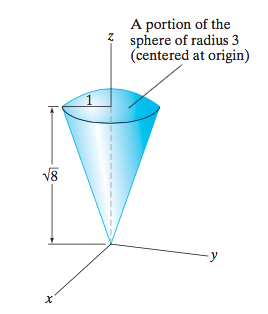
\includegraphics[scale=0.4]{hw6_pic}
\end{center}
\begin{enumerate}
\item Describe the solid, using spherical coordinates.
\[
0\leq\rho\leq3,\ 0\leq\phi\leq\arctan{1\over\sqrt{8}},\ 0\leq\theta\leq2\pi
\]
\item Describe the solid, using cylindrical coordinates.
\[
\sqrt{8}\ r\leq z\leq\sqrt{9-r^{2}},\ 0\leq r\leq 1,\ 0\leq\theta\leq2\pi
\]
\end{enumerate}
\end{enumerate}
\end{document}
